% Options for packages loaded elsewhere
\PassOptionsToPackage{unicode}{hyperref}
\PassOptionsToPackage{hyphens}{url}
\PassOptionsToPackage{dvipsnames,svgnames,x11names}{xcolor}
%
\documentclass[
]{aft}

\usepackage{amsmath,amssymb}
\usepackage{iftex}
\ifPDFTeX
  \usepackage[T1]{fontenc}
  \usepackage[utf8]{inputenc}
  \usepackage{textcomp} % provide euro and other symbols
\else % if luatex or xetex
  \usepackage{unicode-math}
  \defaultfontfeatures{Scale=MatchLowercase}
  \defaultfontfeatures[\rmfamily]{Ligatures=TeX,Scale=1}
\fi
\usepackage{lmodern}
\ifPDFTeX\else  
    % xetex/luatex font selection
\fi
% Use upquote if available, for straight quotes in verbatim environments
\IfFileExists{upquote.sty}{\usepackage{upquote}}{}
\IfFileExists{microtype.sty}{% use microtype if available
  \usepackage[]{microtype}
  \UseMicrotypeSet[protrusion]{basicmath} % disable protrusion for tt fonts
}{}
\makeatletter
\@ifundefined{KOMAClassName}{% if non-KOMA class
  \IfFileExists{parskip.sty}{%
    \usepackage{parskip}
  }{% else
    \setlength{\parindent}{0pt}
    \setlength{\parskip}{6pt plus 2pt minus 1pt}}
}{% if KOMA class
  \KOMAoptions{parskip=half}}
\makeatother
\usepackage{xcolor}
\setlength{\emergencystretch}{3em} % prevent overfull lines
\setcounter{secnumdepth}{-\maxdimen} % remove section numbering
% Make \paragraph and \subparagraph free-standing
\makeatletter
\ifx\paragraph\undefined\else
  \let\oldparagraph\paragraph
  \renewcommand{\paragraph}{
    \@ifstar
      \xxxParagraphStar
      \xxxParagraphNoStar
  }
  \newcommand{\xxxParagraphStar}[1]{\oldparagraph*{#1}\mbox{}}
  \newcommand{\xxxParagraphNoStar}[1]{\oldparagraph{#1}\mbox{}}
\fi
\ifx\subparagraph\undefined\else
  \let\oldsubparagraph\subparagraph
  \renewcommand{\subparagraph}{
    \@ifstar
      \xxxSubParagraphStar
      \xxxSubParagraphNoStar
  }
  \newcommand{\xxxSubParagraphStar}[1]{\oldsubparagraph*{#1}\mbox{}}
  \newcommand{\xxxSubParagraphNoStar}[1]{\oldsubparagraph{#1}\mbox{}}
\fi
\makeatother

\usepackage{color}
\usepackage{fancyvrb}
\newcommand{\VerbBar}{|}
\newcommand{\VERB}{\Verb[commandchars=\\\{\}]}
\DefineVerbatimEnvironment{Highlighting}{Verbatim}{commandchars=\\\{\}}
% Add ',fontsize=\small' for more characters per line
\usepackage{framed}
\definecolor{shadecolor}{RGB}{241,243,245}
\newenvironment{Shaded}{\begin{snugshade}}{\end{snugshade}}
\newcommand{\AlertTok}[1]{\textcolor[rgb]{0.68,0.00,0.00}{#1}}
\newcommand{\AnnotationTok}[1]{\textcolor[rgb]{0.37,0.37,0.37}{#1}}
\newcommand{\AttributeTok}[1]{\textcolor[rgb]{0.40,0.45,0.13}{#1}}
\newcommand{\BaseNTok}[1]{\textcolor[rgb]{0.68,0.00,0.00}{#1}}
\newcommand{\BuiltInTok}[1]{\textcolor[rgb]{0.00,0.23,0.31}{#1}}
\newcommand{\CharTok}[1]{\textcolor[rgb]{0.13,0.47,0.30}{#1}}
\newcommand{\CommentTok}[1]{\textcolor[rgb]{0.37,0.37,0.37}{#1}}
\newcommand{\CommentVarTok}[1]{\textcolor[rgb]{0.37,0.37,0.37}{\textit{#1}}}
\newcommand{\ConstantTok}[1]{\textcolor[rgb]{0.56,0.35,0.01}{#1}}
\newcommand{\ControlFlowTok}[1]{\textcolor[rgb]{0.00,0.23,0.31}{\textbf{#1}}}
\newcommand{\DataTypeTok}[1]{\textcolor[rgb]{0.68,0.00,0.00}{#1}}
\newcommand{\DecValTok}[1]{\textcolor[rgb]{0.68,0.00,0.00}{#1}}
\newcommand{\DocumentationTok}[1]{\textcolor[rgb]{0.37,0.37,0.37}{\textit{#1}}}
\newcommand{\ErrorTok}[1]{\textcolor[rgb]{0.68,0.00,0.00}{#1}}
\newcommand{\ExtensionTok}[1]{\textcolor[rgb]{0.00,0.23,0.31}{#1}}
\newcommand{\FloatTok}[1]{\textcolor[rgb]{0.68,0.00,0.00}{#1}}
\newcommand{\FunctionTok}[1]{\textcolor[rgb]{0.28,0.35,0.67}{#1}}
\newcommand{\ImportTok}[1]{\textcolor[rgb]{0.00,0.46,0.62}{#1}}
\newcommand{\InformationTok}[1]{\textcolor[rgb]{0.37,0.37,0.37}{#1}}
\newcommand{\KeywordTok}[1]{\textcolor[rgb]{0.00,0.23,0.31}{\textbf{#1}}}
\newcommand{\NormalTok}[1]{\textcolor[rgb]{0.00,0.23,0.31}{#1}}
\newcommand{\OperatorTok}[1]{\textcolor[rgb]{0.37,0.37,0.37}{#1}}
\newcommand{\OtherTok}[1]{\textcolor[rgb]{0.00,0.23,0.31}{#1}}
\newcommand{\PreprocessorTok}[1]{\textcolor[rgb]{0.68,0.00,0.00}{#1}}
\newcommand{\RegionMarkerTok}[1]{\textcolor[rgb]{0.00,0.23,0.31}{#1}}
\newcommand{\SpecialCharTok}[1]{\textcolor[rgb]{0.37,0.37,0.37}{#1}}
\newcommand{\SpecialStringTok}[1]{\textcolor[rgb]{0.13,0.47,0.30}{#1}}
\newcommand{\StringTok}[1]{\textcolor[rgb]{0.13,0.47,0.30}{#1}}
\newcommand{\VariableTok}[1]{\textcolor[rgb]{0.07,0.07,0.07}{#1}}
\newcommand{\VerbatimStringTok}[1]{\textcolor[rgb]{0.13,0.47,0.30}{#1}}
\newcommand{\WarningTok}[1]{\textcolor[rgb]{0.37,0.37,0.37}{\textit{#1}}}

\providecommand{\tightlist}{%
  \setlength{\itemsep}{0pt}\setlength{\parskip}{0pt}}\usepackage{longtable,booktabs,array}
\usepackage{calc} % for calculating minipage widths
% Correct order of tables after \paragraph or \subparagraph
\usepackage{etoolbox}
\makeatletter
\patchcmd\longtable{\par}{\if@noskipsec\mbox{}\fi\par}{}{}
\makeatother
% Allow footnotes in longtable head/foot
\IfFileExists{footnotehyper.sty}{\usepackage{footnotehyper}}{\usepackage{footnote}}
\makesavenoteenv{longtable}
\usepackage{graphicx}
\makeatletter
\newsavebox\pandoc@box
\newcommand*\pandocbounded[1]{% scales image to fit in text height/width
  \sbox\pandoc@box{#1}%
  \Gscale@div\@tempa{\textheight}{\dimexpr\ht\pandoc@box+\dp\pandoc@box\relax}%
  \Gscale@div\@tempb{\linewidth}{\wd\pandoc@box}%
  \ifdim\@tempb\p@<\@tempa\p@\let\@tempa\@tempb\fi% select the smaller of both
  \ifdim\@tempa\p@<\p@\scalebox{\@tempa}{\usebox\pandoc@box}%
  \else\usebox{\pandoc@box}%
  \fi%
}
% Set default figure placement to htbp
\def\fps@figure{htbp}
\makeatother

\usepackage{orcidlink}
\definecolor{mypink}{RGB}{219, 48, 122}
\makeatletter
\@ifpackageloaded{caption}{}{\usepackage{caption}}
\AtBeginDocument{%
\ifdefined\contentsname
  \renewcommand*\contentsname{Table of contents}
\else
  \newcommand\contentsname{Table of contents}
\fi
\ifdefined\listfigurename
  \renewcommand*\listfigurename{List of Figures}
\else
  \newcommand\listfigurename{List of Figures}
\fi
\ifdefined\listtablename
  \renewcommand*\listtablename{List of Tables}
\else
  \newcommand\listtablename{List of Tables}
\fi
\ifdefined\figurename
  \renewcommand*\figurename{Figure}
\else
  \newcommand\figurename{Figure}
\fi
\ifdefined\tablename
  \renewcommand*\tablename{Table}
\else
  \newcommand\tablename{Table}
\fi
}
\@ifpackageloaded{float}{}{\usepackage{float}}
\floatstyle{ruled}
\@ifundefined{c@chapter}{\newfloat{codelisting}{h}{lop}}{\newfloat{codelisting}{h}{lop}[chapter]}
\floatname{codelisting}{Listing}
\newcommand*\listoflistings{\listof{codelisting}{List of Listings}}
\makeatother
\makeatletter
\makeatother
\makeatletter
\@ifpackageloaded{caption}{}{\usepackage{caption}}
\@ifpackageloaded{subcaption}{}{\usepackage{subcaption}}
\makeatother

\usepackage[]{natbib}
\bibliographystyle{te}
\usepackage{bookmark}

\IfFileExists{xurl.sty}{\usepackage{xurl}}{} % add URL line breaks if available
\urlstyle{same} % disable monospaced font for URLs
\hypersetup{
  pdftitle={Spatial Autocorrelation},
  pdfauthor={Wei Kang},
  pdfkeywords={Spatial Autocorrelation, Spatial Effects, PySAL, Open
Source},
  colorlinks=true,
  linkcolor={blue},
  filecolor={Maroon},
  citecolor={Blue},
  urlcolor={red},
  pdfcreator={LaTeX via pandoc}}



\title{Spatial Autocorrelation}
\author{
Wei Kang~\orcidlink{0000-0002-1073-7781}\\University of California
Riverside\\\href{mailto:wei.kang@ucr.edu}{wei.kang@ucr.edu}}
\date{}
\begin{document}
\maketitle
\begin{abstract}
Spatial autocorrelation is a key concept in quantitative spatial
analysis that measures the degree of similarity or dissimilarity between
spatially distributed observations. This paper introduces the concept
and measurement of global and local spatial autocorrelation. An
open-source Python workflow is provided to demonstrate how to measure,
visualize, and interpret global and local Moran's I statistics---the
most widely used method for spatial autocorrelation---by analyzing the
spatial patterns of neighborhood housing affordability in the City of
Riverside, California. The workflow includes guidance and code to
address variance instability in proportion variables and the multiple
testing issue in local statistics. Additionally, extensions and
innovations to univariate spatial autocorrelation, such as multivariate
and uncertainty-aware frameworks, are discussed.
\end{abstract}


\section{Introduction}\label{sec-intro}

Spatial autocorrelation is a fundamental concept in quantitative spatial
analysis, providing a framework to measure the degree of similarity or
dissimilarity between spatially distributed observations. This concept
is rooted in Tobler's First Law of Geography, which states: ``Everything
is related to everything else, but near things are more related than
distant things'' \citep{Tobler:1970vs}. Understanding spatial
autocorrelation is critical for examining spatial processes, detecting
spatial patterns, and identifying clusters or outliers within geographic
data \citep{Anselin:2016}.

Spatial autocorrelation can arise for a variety of reasons, including
underlying spatial processes such as diffusion, neighborhood effects, or
spatial spillovers. For example, in housing studies, affordability
patterns may cluster due to shared socioeconomic conditions, policy
interventions, or spatially dependent housing markets. Additionally,
spatial autocorrelation may be induced by data collection or processing.
Specifically, when the unit of observation does not match the unit of
analysis (i.g., mismatched boundaries or the more general more general
modifiable areal unit problem (MANP) \citep{manley2021scale}), spatial
dependencies can arise. This issue may stem from different definitions
of spatial boundaries (e.g., census geographies not aligning with
functional regions) or from measurement errors (e.g., inaccuracies
during map digitization in GIS). In such cases, the spatial structure of
the data may unintentionally introduce spatial autocorrelation.

The presence of spatial autocorrelation has important implications, as
it violates the assumption of independence commonly used in classical
statistical models. Ignoring spatial dependence may lead to biased
estimates, inefficient models, or incorrect statistical inferences.
Recognizing and quantifying spatial autocorrelation, therefore, is
essential for accurate analysis, policy design, and decision-making.

While the concept of spatial autocorrelation and its measurements has
been extensively discussed in many textbooks and journal articles
\citep{OSullivan:2010, de2007geospatial, bivand2013applied, rey2023geographic},
this paper adds to the field by providing a practical and interactive
example of its implementation. Using open-source Python packages, this
notebook explores the spatial distribution of neighborhood housing
affordability in the City of Riverside of Inlanda Southern California.
The analysis applies both global Moran's I to measure overall spatial
autocorrelation and local Moran's I to identify spatial clusters and
outliers, offering a reproducible workflow for spatial autocorrelation
analysis.

This notebook is organized into several sections. It begins with an
introduction to the computational environment and data, outlining the
tools and datasets used for analysis. The data section details the
sources and preprocessing steps necessary for the analysis. The next
section introduces the concept of spatial autocorrelation and provides a
basic conceptual understanding. This is followed by a demonstration of
spatial autocorrelation analysis applied to the housing affordability
dataset, featuring visualizations and statistical insights. The notebook
concludes with a summary of recent developments in spatial
autocorrelation analysis.

\section{Computational environment}\label{sec-ce}

A wide array of specialized sopen source oftware are available for
carrying out spatial autocorrelation analysis, including \texttt{spdep}
(R) \citep{Pebesma2023}, \texttt{esda}/\texttt{pysal} (Python)
\citep{pysal2007}, and \texttt{rgeoda} (R) and \texttt{pygeoda} (python)
which are based on \texttt{libgeoda} (C++), the core of the widely-used
Graphic User Interface (GUI)-based software \texttt{GeoDa}
\citep{Anselin20221}. The choice would be much of a personal preference
as they are all open source, easy to be integrated into a computational
workflow, and producing similar output with only minor differences
\citep{Bivand2022}.

In this computational notebook, I will work in a Python 3 environment
and rely on Python Spatial Analysis Library (PySAL), a mainstay
open-source Python ecosystem for spatial data science
\citep{Kang:2020c}, to demonstrate spatial autocorrelation analysis.
Within the ecosystem, \texttt{pysal} is a meta package pulling together
about 20 subpackages in the ecosystem capable of conducting a
comprehensive variety of spatial analyses, including exploratory spatial
data analysis (ESDA), spatial regressions, and spatial optimization
\citep{Rey2022}. The subpackages are more lightweighted and can be
installed and used independently to accomplish specific spatial analysis
tasks. In this notebook, I will mainly work with \texttt{esda} and
\texttt{libpysal}, two of the subpackages in the PySAL ecosystem, which
are sufficient for the demonstration needs: \texttt{esda} includes a
variety of classic and state-of-the-art global and local spatial
autocorrelation statistics; \texttt{libpysal} is the foundation of all
the other subpackages in the PySAL ecosystem, which inclueds
foundational algorithms and data structures needed for spatial analysis,
such as the construction of various spatial weights. I will also draw on
functionalities of \texttt{splot}, a light-weight visualization package
in the PySAL ecosystem for generating statistical plots assisting the
undertanding of the results of the spatial autocorrelation analysis
\citep{Lumnitz2020}. For the complete workflow, I will use
\texttt{geopandas} for spatial data reading and wrangling
\citep{joris_van_den_bossche_2024_12625316}, \texttt{libpysal} for
constructing spatial weights, \texttt{esda} for the estimation and
inference of global and local spatial autocorrelation, \texttt{splot},
\texttt{matplotlib}, and \texttt{contextily} for statistical and
geospatial visualization, and the built-in python module \texttt{random}
to ensure replication and reproducibility of the inference results.

In the code cell below, all the required python packages, classes, and
functions are imported:

\begin{Shaded}
\begin{Highlighting}[]
\CommentTok{\# loading packages for spatial data manipulation and analysis }
\ImportTok{import}\NormalTok{ geopandas }\ImportTok{as}\NormalTok{ gpd}
\ImportTok{import}\NormalTok{ libpysal}
\ImportTok{import}\NormalTok{ esda}

\CommentTok{\# loading visualization packages}
\ImportTok{from}\NormalTok{ splot.esda }\ImportTok{import}\NormalTok{ lisa\_cluster}
\ImportTok{import}\NormalTok{ matplotlib.pyplot }\ImportTok{as}\NormalTok{ plt}
\ImportTok{import}\NormalTok{ contextily}

\CommentTok{\# python built{-}in module for generating pseudo{-}random numbers }
\CommentTok{\# of permutation based inference}
\ImportTok{import}\NormalTok{ random}

\CommentTok{\# python package for scientific computing }
\ImportTok{import}\NormalTok{ numpy }\ImportTok{as}\NormalTok{ np}

\CommentTok{\# printing the name/version of all imported modules}
\CommentTok{\#\%load\_ext watermark}
\CommentTok{\#\%watermark {-}{-}iversions }
\end{Highlighting}
\end{Shaded}

\section{Data}\label{sec-data}

Both the geographies and attributes used in this analysis are sourced
from the U.S. Census Bureau for the investigation of the spatial
patterns of neighborhood housing affordability in the City of Riverside,
CA. onsistent with the literature, neighborhoods are represented by
census tracts, and tract polygons are sourced from the 2020 Census
Bureau's TIGER/Line Shapefiles\footnote{Census 2020 TIGER/Line
  Shapefiles:
  https://www.census.gov/geographies/mapping-files/time-series/geo/tiger-line-file.2020.html}.
A total of 93 tract polygons are included as they either fall within or
intersect the city boundary.

The primary attribute of interest is the proportion of housholds that
are burdened by housing costs. Specifically, households spending 30\% or
more of their gross incomes on housing costs, which could include rent
or mortgage payments, utilities, and related expenses, are considered
housing cost-burdened. This definition of housing affordability focuses
on the ability of households to afford housing without experiencing
financial strain and has been widely adopted by government agencies
(e.g., the U.S. Department of Housing and Urban Development (HUD)) and
affordable housing programs (e.g., HUD's Housing Choice Voucher
Program).

The dataset includes three continuous attributes related to housing cost
burden, derived from the 2018--2022 5-year American Community Survey
(ACS) estimates: (1) \texttt{All30C}: the number of housing
cost-burdened households. (2) \texttt{AllC}: the total number of
households in the tract. (3) \texttt{All30P}: the proportion of housing
cost-burdened households, calculated as All30C divided by AllC.

These variables reflect all households, including renters and
homeowners, with and without a mortgage.

A Jupyter Notebook (Python) named ``DataCollection'' is included in the
repository. It demonstrates how to use the Census API to query the
source data (i.e., ACS and TIGER/Line Shapefiles) and perform the
necessary transformations, calculations, and merges.

The analysis begins by reading the spatial data file and projecting the
geographic coordinate system to a planar coordinate system that uses
linear measurements for the coordinates.

\begin{Shaded}
\begin{Highlighting}[]
\CommentTok{\# read the spatial data set (shapefile) as a GeoDataframe}
\NormalTok{gdf }\OperatorTok{=}\NormalTok{ gpd.read\_file(}\StringTok{"data/CostBurden\_Riverside.shp"}\NormalTok{)}

\CommentTok{\# set the projected coordinate system}
\NormalTok{gdf }\OperatorTok{=}\NormalTok{ gdf.to\_crs(}\StringTok{"epsg:2770"}\NormalTok{)}

\NormalTok{gdf.info()}
\end{Highlighting}
\end{Shaded}

\begin{verbatim}
<class 'geopandas.geodataframe.GeoDataFrame'>
RangeIndex: 93 entries, 0 to 92
Data columns (total 5 columns):
 #   Column    Non-Null Count  Dtype   
---  ------    --------------  -----   
 0   GEOID     93 non-null     object  
 1   AllC      93 non-null     int64   
 2   All30C    93 non-null     int64   
 3   All30P    92 non-null     float64 
 4   geometry  93 non-null     geometry
dtypes: float64(1), geometry(1), int64(2), object(1)
memory usage: 3.8+ KB
\end{verbatim}

\section{Basic conceptual intuition}\label{sec-intuition}

When our research question involves spatial entities, one of the first
steps is often to visualize the attribute of interest on a map. From the
map, we could visually identify where the high and low values occur.
Most often than not, these patterns are not spatially random. In other
words, areas with low values are more likely to be surrounded by other
low values, and similarly for high values. This type of spatial
association is referred to as spatial dependence, which invalidates the
assumption of independence commonly used in classical statistical
models. Consequently, it is important to determine whether the observed
spatial pattern is significant---that is, whether it deviates from what
would be expected under spatial randomness.

Spatial autocorrelation statistics were developed for this purpose.
These statistics measure the correlation of an attribute across space by
simultaneously evaluating locational and attribute similarity.
Observations that are similar in attribute values and geographically
close contribute positively to spatial autocorrelation statistics.
Conversely, observations that are dissimilar in attribute values but
geographically close contribute negatively.

Global spatial autocorrelation (GSA) statistics are summary measures
produced for the entire map, indicating the extent to which higher (or
lower) values are overall geographically clustered. They work by
assessing locational and attribute similarities across all pairs of
observations. A generic form of a GSA statistic is given by Equation
(\ref{e1}):

\begin{equation}
\label{e1}
\Gamma = \sum_i \sum_j w_{ij} y_{ij} 
\end{equation}

where \(\Gamma\) is a GSA statistic, \(Y\) is a matrix of attribute
similarity, and \(W\) is a matrix representing locational similarity.
Different functions have been proposed to measure attribute similarity
for continuous values, leading to various GSA statistics, such as
Moran's I and Geary's C. The matrix \(W\), known as the spatial weights
matrix, encodes our perception about spatial relationships between
observations. The weights in \(W\) can be based on contiguity, distance,
or accessibility.\\
Only the elements of \(W\) that correspond to pairs of neighboring
observations take non-zero values, making it a sparse matrix even for
moderately large datasets. For instance, with a queen-based contiguity
weight for polygon geometries, two observations (\(i \neq j\)) are
considered neighbors if they share a vertex or an edge and the \((i,j)\)
entry in \(W\) is nonzero.

In addition to summarizing spatial autocorrelation across the entire map
using a single statistic, it is often important to identify spatial
clusters of high or low values, commonly referred to as spatial hotpots
and coldspots. Additionally, spatial outliers, defined defined as low
(high) values surrounded by high (low) values, may also be of interest.
Local spatial autocorrelation (LSA) statistics, which are local
decompositions of GSA statistics, are designed for such purposes. LSA
statistics provide a measure of spatial autocorrelation for each
observation by using information from neighboring observations This
approach reveals the spatial nonstationarity of spatial autocorrelation,
meaning that even in the absence of significant global spatial
autocorrelation, local pockets of strong spatial autocorrelation may
still exist. A generic form of an LSA statistic is given by Equation
(\ref{e2}):

\begin{equation}
\label{e2}
\Gamma_i = \sum_j w_{ij} y_{ij}
\end{equation}

where \(\Gamma_i\) is the LSA statistic for observation \(i\). Similar
to the GSA statistics, different LSA statistics exist based on various
definitions of attribute similarity. For instance, local Moran's I and
local Geary's C are local decompositions of Moran's I and Geary's C,
respectively\citep{Anselin:1995fn}.

\section{Application}\label{sec-app}

In this section, I will demonstrate how to analyze the spatial
distribution of neighborhood housing affordability in the City of
Riveride using gloabl and local Moran's Is, the most widely used methods
for assessing global and local spatial autocorrelation. These statistics
measures spatial autocorrelation by utilizing deviations from the mean
to define attribute similarity. Local Moran's I evaluates the
coexistence of attribute and locational similarity by multipling the
focal unit's deviation and by spatial lag, which is the average of the
deviations of its neighbors as defined in the spatial weights matrix
\citep{Anselin:1995fn}. Global Moran's I is proportional to the
summation of Local Moran's Is. A positive estimate for global (local)
Moran's I suggest positive gloabl (local) spatial autocorrelation,
meaning that similar values (high or low) are geographically clustered.
The larger the estimate, the stronger the spatial autocorrelation.
Conversely, a large negative estimate indicates negative spatial
autocorrelation, where dissimilar values (e.g., high values surrounded
by low values) are more likely to be near each other.

Since we are interested in the spatial patterns of a proportion
variable, proper adjustment are necessary to address its intrinsic
variance instability. Specifically, census tracts with a smaller number
of households tend to have lower precision in their rate estimates,
which could lead to the incorrect identification of spurious outliers.

\subsection{Choropleth mapping of the spatial
pattern}\label{choropleth-mapping-of-the-spatial-pattern}

The first step of the ESDA is often to visually inspect the spatial
distribution. As mentioned earlier, the raw rate, calculated by dividing
the number of cost-burdened households by the total number of
households, suffer from variance instability. One way to address this
issue is by applying Empirical Bayes (EB) smoothing, where the EB rate
is the weighted average between the raw rate and the citywide average,
with larger weights given to the city average for tracts with a smaller
number of households. The function \texttt{Empirical\_Bayes} from
\texttt{esda}'s \texttt{smoothing} can be used to easily estimate the EB
rates. The estimated EB rate will be added to the dataset as a new
column named \texttt{All30EBP}.

\begin{Shaded}
\begin{Highlighting}[]
\NormalTok{gdf\_temp }\OperatorTok{=}\NormalTok{ gdf[gdf.AllC}\OperatorTok{\textgreater{}}\DecValTok{0}\NormalTok{]}
\NormalTok{gdf\_temp}\OperatorTok{=}\NormalTok{ gdf\_temp.assign(}
\NormalTok{  All30EBP}\OperatorTok{=}\NormalTok{esda.smoothing.Empirical\_Bayes(}
\NormalTok{    gdf\_temp.All30C.values, }
\NormalTok{    gdf\_temp.AllC.values).r)}

\NormalTok{gdf }\OperatorTok{=}\NormalTok{ gdf.set\_index(}\StringTok{"GEOID"}\NormalTok{).merge(}
\NormalTok{  gdf\_temp[[}\StringTok{"All30EBP"}\NormalTok{,}\StringTok{"GEOID"}\NormalTok{]].set\_index(}\StringTok{"GEOID"}\NormalTok{),}
\NormalTok{  how}\OperatorTok{=}\StringTok{"outer"}\NormalTok{, }
\NormalTok{  right\_index}\OperatorTok{=}\VariableTok{True}\NormalTok{, }
\NormalTok{  left\_index}\OperatorTok{=}\VariableTok{True}\NormalTok{)}
\end{Highlighting}
\end{Shaded}

Next, we visualize the raw rate map and the EB rate map side-by-side for
comparison. We use call the \texttt{plot()} method from
\texttt{GeoDataFrame} to produce a choropleth map with quintile
classification, providing a quick preview of the spatial distribution of
the housing cost-burden rate across neighborhoods in the City of
Riverside. Additionally, a basemap could be overlaid on the choropleth
map to give geographic context to the study area using the
\texttt{contextily} package.

\begin{Shaded}
\begin{Highlighting}[]
\NormalTok{f, axes }\OperatorTok{=}\NormalTok{ plt.subplots(}\DecValTok{1}\NormalTok{,}\DecValTok{2}\NormalTok{, figsize}\OperatorTok{=}\NormalTok{(}\DecValTok{20}\NormalTok{, }\DecValTok{10}\NormalTok{))}
\NormalTok{gdf.plot(}
  \StringTok{"All30P"}\NormalTok{, }
\NormalTok{  cmap}\OperatorTok{=}\StringTok{"YlGn"}\NormalTok{, }
\NormalTok{  k}\OperatorTok{=}\DecValTok{5}\NormalTok{, }
\NormalTok{  scheme}\OperatorTok{=}\StringTok{\textquotesingle{}quantiles\textquotesingle{}}\NormalTok{, }
\NormalTok{  edgecolor}\OperatorTok{=}\StringTok{"white"}\NormalTok{,}
\NormalTok{  linewidth}\OperatorTok{=}\DecValTok{1}\NormalTok{,}
\NormalTok{  alpha}\OperatorTok{=}\FloatTok{0.75}\NormalTok{, }
\NormalTok{  legend}\OperatorTok{=}\VariableTok{True}\NormalTok{, }
\NormalTok{  ax}\OperatorTok{=}\NormalTok{axes[}\DecValTok{0}\NormalTok{], }
\NormalTok{  missing\_kwds}\OperatorTok{=}\NormalTok{\{}
    \StringTok{"color"}\NormalTok{: }\StringTok{"lightgrey"}\NormalTok{,}
    \StringTok{"label"}\NormalTok{: }\StringTok{"No population"}
\NormalTok{    \}}
\NormalTok{  )}
\NormalTok{contextily.add\_basemap(}
\NormalTok{  axes[}\DecValTok{0}\NormalTok{],}
\NormalTok{  crs}\OperatorTok{=}\NormalTok{gdf.crs, }
\NormalTok{  source}\OperatorTok{=}\NormalTok{contextily.providers.Esri.WorldTopoMap}
\NormalTok{  )}
\NormalTok{axes[}\DecValTok{0}\NormalTok{].set\_title(}\StringTok{"Raw rate map"}\NormalTok{)}
\NormalTok{axes[}\DecValTok{0}\NormalTok{].set\_axis\_off()}\OperatorTok{;}

\NormalTok{gdf.plot(}
  \StringTok{"All30EBP"}\NormalTok{, }
\NormalTok{  cmap}\OperatorTok{=}\StringTok{"YlGn"}\NormalTok{, }
\NormalTok{  k}\OperatorTok{=}\DecValTok{5}\NormalTok{, }
\NormalTok{  scheme}\OperatorTok{=}\StringTok{\textquotesingle{}quantiles\textquotesingle{}}\NormalTok{, }
\NormalTok{  edgecolor}\OperatorTok{=}\StringTok{"white"}\NormalTok{,}
\NormalTok{  linewidth}\OperatorTok{=}\DecValTok{1}\NormalTok{,}
\NormalTok{  alpha}\OperatorTok{=}\FloatTok{0.75}\NormalTok{, }
\NormalTok{  legend}\OperatorTok{=}\VariableTok{True}\NormalTok{, }
\NormalTok{  ax}\OperatorTok{=}\NormalTok{axes[}\DecValTok{1}\NormalTok{], }
\NormalTok{  missing\_kwds}\OperatorTok{=}\NormalTok{\{}
    \StringTok{"color"}\NormalTok{: }\StringTok{"lightgrey"}\NormalTok{,}
    \StringTok{"label"}\NormalTok{: }\StringTok{"No population"}
\NormalTok{    \}}
\NormalTok{  )}
\NormalTok{contextily.add\_basemap(}
\NormalTok{  axes[}\DecValTok{1}\NormalTok{],}
\NormalTok{  crs}\OperatorTok{=}\NormalTok{gdf.crs, }
\NormalTok{  source}\OperatorTok{=}\NormalTok{contextily.providers.Esri.WorldTopoMap}
\NormalTok{  )}
\NormalTok{axes[}\DecValTok{1}\NormalTok{].set\_title(}\StringTok{"EB rate map"}\NormalTok{)}
\NormalTok{axes[}\DecValTok{1}\NormalTok{].set\_axis\_off()}\OperatorTok{;}
\end{Highlighting}
\end{Shaded}

\pandocbounded{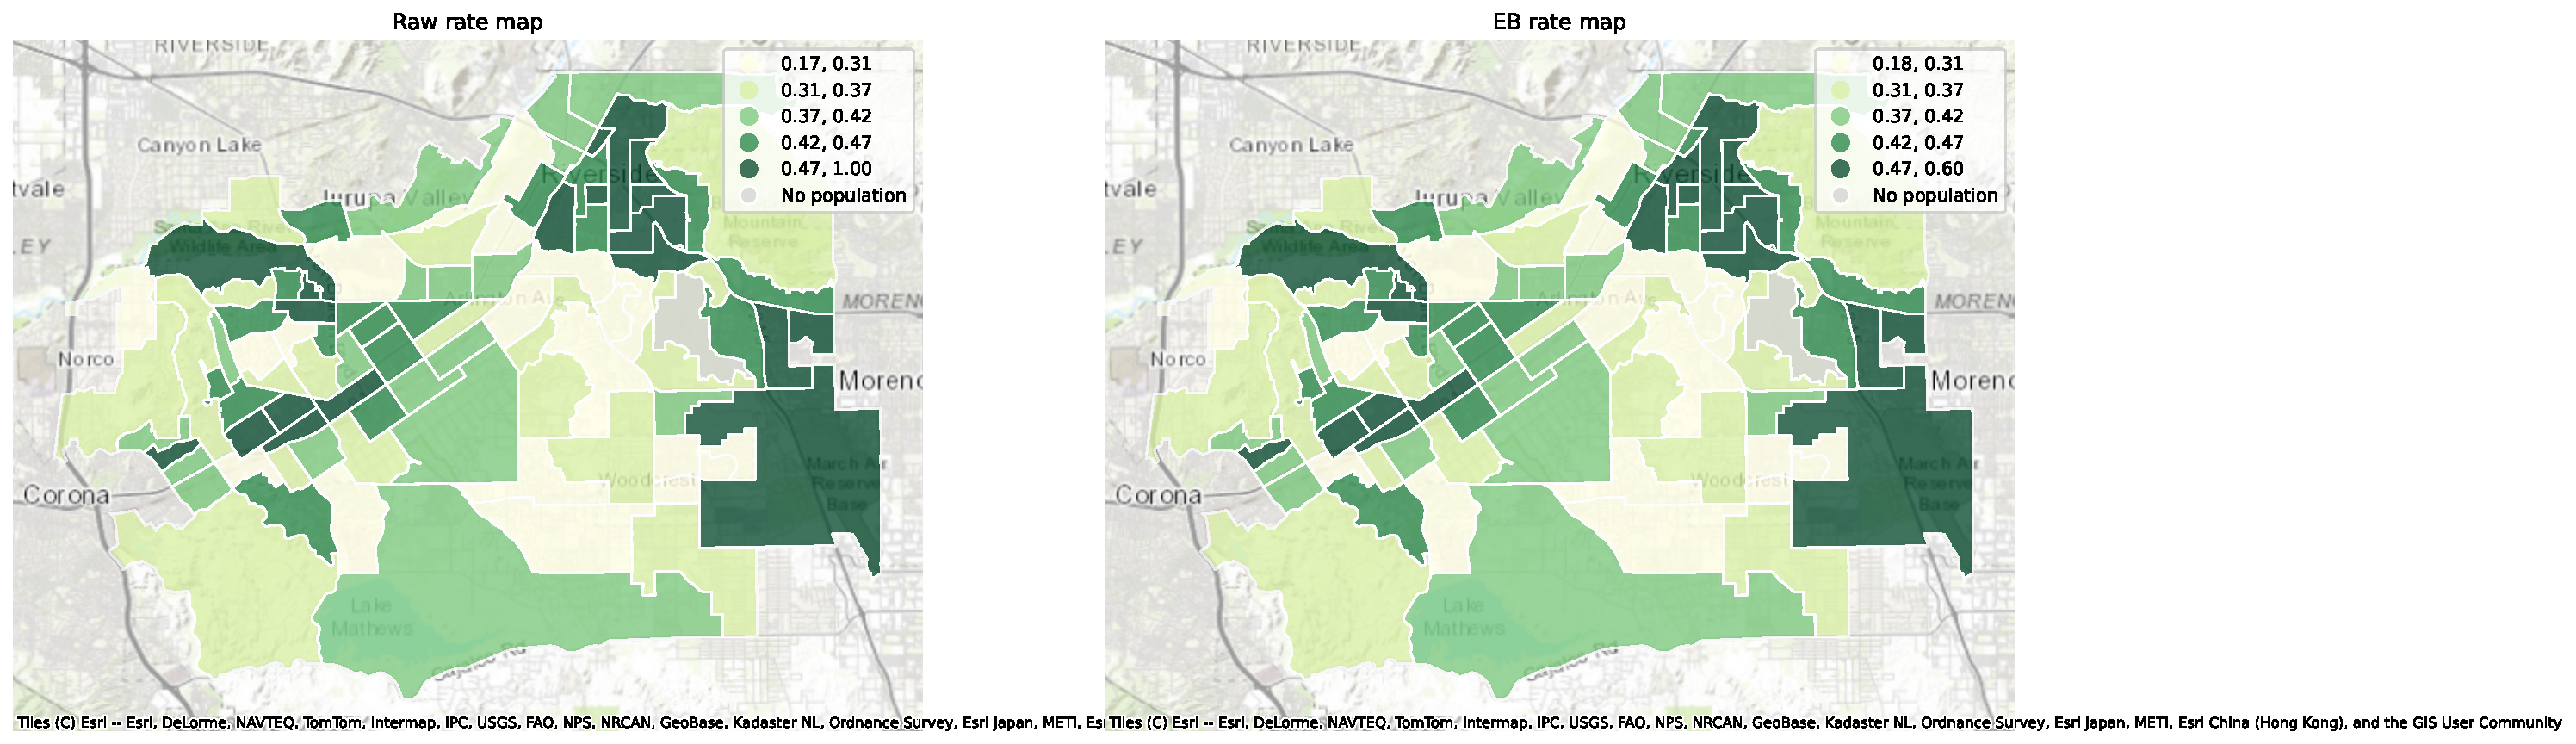
\includegraphics[keepaspectratio]{article_files/figure-pdf/cell-5-output-1.pdf}}

The general spatial patterns are similar across the raw and EB rate maps
despite small differences in the range of rates. Visually, neighborhoods
with similar values seem to be geographically close. For instance,
neighborhoods that were more prevalent with housing cost-burdened
households are concentrated in the northeastern and western parts of the
city, as well as the southeastern neighborhoods that overlap
significantly with the City of Moreno Valley. In contrast, lower rates
concentrated in southern Riverside, which are known for newer
developments and suburban-style housing. However, our visual preception
could be deceiving, which is particularly relevant as the polygons vary
in size. We therefore adopt spatial autocorrelation methods to formally
test aganist spatial randomness and identify local hot/cold spots and
outliers.

\subsection{Spatial autocorrelation
analysis}\label{spatial-autocorrelation-analysis}

In \texttt{esda}, the estimation and inference of the spatial
autocorrelation statistics, global and local Moran's Is, are implemented
as the respective Python \texttt{classes}: \texttt{Moran} and
\texttt{Moran\_Local}. For each, locational similarity (i.e., spatial
weights) must be defined and calculated prior to instantiation of these
classes whereas attribute similarity is assessed internally, making
attribute data a required parameter. As we are analyzing proportion
variable which could suffer from variance instability, the Empirical
Bayes (EB) standardization has been proposed to correct Moran's I
statistics as a solution \citep{SIM:SIM179}. The \texttt{esda} classes
\texttt{Moran\_Rate} and \texttt{Moran\_Rate\_Local} implemented this
adjustment. In contrast to \texttt{Moran} and \texttt{Moran\_Local}
where the attribute of interest should be provided, these two classes
require values for the number of the events (i.e., housing cost-burdened
households) and the population at risk (i.e., total households).

\subsubsection{Locational similarity and spatial
weights}\label{locational-similarity-and-spatial-weights}

The first step of spatial autocorrelation analysis is to construct
spatial weights for representing locational similarity. In this
application, a queen contiguity spatial weight matrix will be
constructed using \texttt{esda}'s newest module, \texttt{graph}, a
modern implementation of spatial weights \citep{pysalGraphMigration}.

\begin{Shaded}
\begin{Highlighting}[]
\CommentTok{\#tracts without any population are removed before the analysis}
\NormalTok{gdf\_r }\OperatorTok{=}\NormalTok{ gdf[gdf.AllC}\OperatorTok{\textgreater{}}\DecValTok{0}\NormalTok{] }

\CommentTok{\# construct queen{-}based spatial weights }
\NormalTok{g\_queen }\OperatorTok{=}\NormalTok{ libpysal.graph.Graph.build\_contiguity(gdf\_r, rook}\OperatorTok{=}\VariableTok{False}\NormalTok{)}
\end{Highlighting}
\end{Shaded}

We can call its adjacency attribute to inspect the neighbor information
for each tract:

\begin{Shaded}
\begin{Highlighting}[]
\NormalTok{g\_queen.adjacency }
\end{Highlighting}
\end{Shaded}

\begin{verbatim}
focal        neighbor   
06065030101  06065030103    1
             06065030104    1
             06065030502    1
             06065042209    1
             06065042300    1
                           ..
06065050901  06065046700    1
             06065050902    1
06065050902  06065042206    1
             06065042212    1
             06065050901    1
Name: weight, Length: 528, dtype: int64
\end{verbatim}

The returned value is a \texttt{pandas} multi-index Series. For each
focal tract, the second index lists tracts that share a vertex or edge,
which are its queen-contiguity neighbors, and the last column (value of
the Series) is the corresponding weight for each neighbor. In the
queen-contiguity spatial weight, every weight has the value of 1.

Futher, we need to row-standardize the spatial weight matrix for the
estimation of the global and local Moran's I statistics. This can be
accomplished by calling the \texttt{transform} method and passing a
\texttt{string} value of \texttt{"r"} on the \texttt{graph} object.
After the transformation, for each focal tract, the weights sum up to 1.

\begin{Shaded}
\begin{Highlighting}[]
\NormalTok{gr }\OperatorTok{=}\NormalTok{ g\_queen.transform(}\StringTok{"r"}\NormalTok{)}
\NormalTok{gr.adjacency}
\end{Highlighting}
\end{Shaded}

\begin{verbatim}
focal        neighbor   
06065030101  06065030103    0.200000
             06065030104    0.200000
             06065030502    0.200000
             06065042209    0.200000
             06065042300    0.200000
                              ...   
06065050901  06065046700    0.200000
             06065050902    0.200000
06065050902  06065042206    0.333333
             06065042212    0.333333
             06065050901    0.333333
Name: weight, Length: 528, dtype: float64
\end{verbatim}

\subsubsection{Estimation and inference}\label{estimation-and-inference}

The discussion so far has been focused on the estimation of spatial
autocorrelation statistics. While a large positive Moran's I statistic
suggests a tendency for high (low) values to cluster near other high
(low) values, formal inference is required to reject spatial
randomness---the null hypothesis of GSAs.

Both analytical and permutation-based approaches have been proposed for
inference regarding Moran's I. he analytical approach, which assumes
independent and normally distributed random variates under the null
hypothesis, is straightforward to implement. However, it relies on
assumptions of normality, spatial stationarity, and a sufficiently large
sample size, all of which are easily violated in practice.

In contrast, the permutation-based approach is more robust, as it does
not require these assumptions. Instead, it constructs a reference
distribution for Moran's I by repeatedly permuting the observed values
across locations. From this reference distribution, a pseudo p-value is
calculated to assess the significance of the observed Moran's I.

For local Moran's I, conditional random permutation is performed, where
the value of the focal tract remains fixed while the values of other
observations are spatially permuted. This process generates a unique
reference distribution for each tract, which is then used to calculate
its corresponding pseudo p-value. The inference of local Moran's Is
would potentially suffer from multiple testing issues as we are
conducting a lot of tests (i.e., number of observations) simultaneously.
By random chance, 5\% of tests would be rejected at the 5\% significance
level. While several methods for addressing multiple testing have been
proposed, the False Discovery Rate (FDR) method is employed in this
demonstration \citep{Benjamini2001, Castro:2006tz}.

\paragraph{Global Spatial
autocorrelation}\label{global-spatial-autocorrelation}

The \texttt{esda} classes are designed in such manner that estimation
and inference are simutaneously conducted. For the permutation-based
inference, we need to set the desired number of (conditional) random
spatial permutations. The number of permutations to be 99999 to be
consistent across global and local inference as the local inference
requires the number of permutations to be sufficiently large to yield a
pseudo p-value that is small enough once the multiple testing is
adjusted for with the FDR method.

\begin{Shaded}
\begin{Highlighting}[]
\CommentTok{\# initialize the random number generator with a given seed to make sure }
\CommentTok{\# the permutation based inference can be replicated on different computers }
\CommentTok{\# and at different times}
\NormalTok{random.seed(}\DecValTok{5}\NormalTok{)}

\CommentTok{\# create an instance of the Moran class from esda}
\NormalTok{moran }\OperatorTok{=}\NormalTok{ esda.Moran\_Rate(}
\NormalTok{  gdf\_r.All30C.values, }
\NormalTok{  gdf\_r.AllC.values,  }
\NormalTok{  gr, }
\NormalTok{  permutations}\OperatorTok{=}\DecValTok{99999}\NormalTok{)}

\BuiltInTok{print}\NormalTok{(}\StringTok{"Moran\textquotesingle{}s I estimate:"}\NormalTok{, moran.I)}
\BuiltInTok{print}\NormalTok{(}\StringTok{"Peudo p{-}value:"}\NormalTok{, moran.p\_sim)}
\end{Highlighting}
\end{Shaded}

\begin{verbatim}
Moran's I estimate: 0.34004457985355707
Peudo p-value: 1e-05
\end{verbatim}

The estimate of Moran's I statitic is a positive 0.34. The peudo p-value
under 99,999 permutations is 1e-05, meaning that none of the permuted
spatial pattern yielded a statistic larger than the actual observed
data. These results indicate a strong deviation from spatial randomness
in neighborhood housing affordability. In other words, neighborhoods
with higher (or lower) concentrations of cost-burdened households were
more likely to be adjacent to similar neighborhoods.

\paragraph{Local spatial
autocorrelation}\label{local-spatial-autocorrelation}

Next, we use local Moran's I to decompose the global statistic and to
detect potential hot/cold spots or spatial outliers. The instantiation
of the local Moran class is similar to that for the global class:

\begin{Shaded}
\begin{Highlighting}[]
\NormalTok{random.seed(}\DecValTok{5}\NormalTok{)}

\CommentTok{\# create an instance of the Moran\_Local class from esda}
\NormalTok{moran\_loc }\OperatorTok{=}\NormalTok{ esda.moran.Moran\_Local\_Rate(}
\NormalTok{  gdf\_r.All30C.values, }
\NormalTok{  gdf\_r.AllC.values, }
\NormalTok{  g\_queen, }
\NormalTok{  transformation }\OperatorTok{=} \StringTok{"r"}\NormalTok{,}
\NormalTok{  permutations}\OperatorTok{=}\DecValTok{99999}
\NormalTok{  )}
\NormalTok{moran\_loc.Is.}\BuiltInTok{round}\NormalTok{(}\DecValTok{2}\NormalTok{)}
\end{Highlighting}
\end{Shaded}

\begin{verbatim}
array([ 0.31, -0.02, -0.03,  0.14, -0.02, -0.26,  0.26,  0.52,  1.36,
        0.67,  0.53,  0.27,  0.88, -0.05,  0.15, -0.26, -0.02,  0.02,
        0.01,  0.4 , -0.05, -0.  , -0.  ,  0.07,  0.1 ,  0.22,  0.27,
       -0.01,  0.05, -0.14,  0.12,  0.01, -0.05, -0.14, -0.03,  0.02,
        0.39, -0.1 , -0.02, -0.  ,  0.11, -0.03,  0.  ,  0.  ,  1.45,
        0.25, -0.43,  0.01,  0.31, -0.1 , -0.04, -0.26,  0.07,  0.26,
       -0.03,  0.02,  0.09, -0.16,  0.15,  0.49,  0.16, -0.13,  0.24,
       -0.26,  0.26,  0.83,  0.45,  0.5 , -0.08,  0.26,  0.02,  1.28,
        1.97,  1.38,  1.22,  0.08,  1.14,  2.02,  1.69,  1.8 ,  0.25,
        0.85, -0.76, -0.04, -0.06,  0.98,  0.74,  3.69,  3.93, -1.26,
        0.22, -0.13])
\end{verbatim}

As shown above, for each neighborhood, a local Moran's I statistic was
estimated and these values vary - some are larger than the global
Moran's I estimate of 0.34 and others are smaller. A choropleth map of
the local statistics would be useful for understanding which
neighborhoods have larger and smaller local spatial autocorrelation:

\begin{Shaded}
\begin{Highlighting}[]
\CommentTok{\# add local Moran\textquotesingle{}s I estimates as a new column }
\CommentTok{\# named "lisa" to the GeoDataFrame}
\NormalTok{gdf\_r }\OperatorTok{=}\NormalTok{ gdf\_r.assign(lisa}\OperatorTok{=}\NormalTok{moran\_loc.Is)}

\NormalTok{f, ax }\OperatorTok{=}\NormalTok{ plt.subplots(}\DecValTok{1}\NormalTok{,}\DecValTok{1}\NormalTok{, figsize}\OperatorTok{=}\NormalTok{(}\DecValTok{10}\NormalTok{, }\DecValTok{7}\NormalTok{))}
\NormalTok{gdf\_r.plot(}
  \StringTok{"lisa"}\NormalTok{, }
\NormalTok{  cmap}\OperatorTok{=}\StringTok{"coolwarm"}\NormalTok{, }
\NormalTok{  k}\OperatorTok{=}\DecValTok{5}\NormalTok{, }
\NormalTok{  scheme}\OperatorTok{=}\StringTok{\textquotesingle{}quantiles\textquotesingle{}}\NormalTok{, }
\NormalTok{  edgecolor}\OperatorTok{=}\StringTok{"white"}\NormalTok{,}
\NormalTok{  linewidth}\OperatorTok{=}\DecValTok{1}\NormalTok{,}
\NormalTok{  alpha}\OperatorTok{=}\FloatTok{0.75}\NormalTok{, }
\NormalTok{  legend}\OperatorTok{=}\VariableTok{True}\NormalTok{, }
\NormalTok{  ax}\OperatorTok{=}\NormalTok{ax}
\NormalTok{  )}

\NormalTok{contextily.add\_basemap(}
\NormalTok{  ax,}
\NormalTok{  crs}\OperatorTok{=}\NormalTok{gdf\_r.crs, }
\NormalTok{  source}\OperatorTok{=}\NormalTok{contextily.providers.Esri.WorldTopoMap}
\NormalTok{  )}\OperatorTok{;}
\NormalTok{ax.set\_title(}\StringTok{"Local Moran\textquotesingle{}s I Estimates"}\NormalTok{)}\OperatorTok{;}
\NormalTok{ax.set\_axis\_off()}\OperatorTok{;}
\end{Highlighting}
\end{Shaded}

\pandocbounded{\includegraphics[keepaspectratio]{article_files/figure-pdf/cell-11-output-1.pdf}}

As shown in the map, large positive values clustered in the northeastern
and central city - an indication of potential hot or cold spots
depending on the housing affordability levels of the focal tract.
Additionally, despite the positive estimate obtained for the global
measure, some neighborhoods exhibited negative local spatial
autocorrelation, an indication of low (high) levels of housing
affordability being surrounded by high (low) levels of housing
affordability, or spatial outliers.

In order to determine whether our visual perception is statistically
sound, we resort to the peudo p-values obtained for each tract with
conditional spatial permutation. As described before, we adjust for
multiple local testing with FDR. The adjusted threshold for the overall
5\% significance level could be calculated using \texttt{esda}'s
function \texttt{fdr}:

\begin{Shaded}
\begin{Highlighting}[]
\NormalTok{p\_adj }\OperatorTok{=}\NormalTok{ esda.fdr(moran\_loc.p\_sim, }\FloatTok{0.05}\NormalTok{)}
\BuiltInTok{print}\NormalTok{(p\_adj)}
\end{Highlighting}
\end{Shaded}

\begin{verbatim}
0.004891304347826087
\end{verbatim}

The adjusted threshold of 0.005 is much smaller than 0.05. Next, we used
this threshold to conduct inference about the local Moran's I
statistics, which could be accomplished by calling the method
\texttt{get\_cluster\_labels()} from the \texttt{Moran\_Local\_Rate}
instance and passing the adjusted threshold. This method could generate
one of five unique values for each neighborhoods: Insignificant,
High-High, Low-Low, Low-High, and High-Low. Apart from
``Insignificant'', the last four values indicate statistically
significant local statistics with the family significance level of 5\%.
Additionally, for these four values, the value on the left of \texttt{-}
refers to the attribute level of the focal unit, whether it is larger
(i.e., High) or smaller (i.e., Low) than the global average; similarly,
the value on the right of \texttt{-} refers to the attribute level of
the spatial lag of the focal unit - in other words, whether the average
of the neighboring units is larger (i.e., High) or smaller (i.e., Low)
than the global average of all spatial lags. Following these
definitions, High-High and Low-Low are indicators of hot and cold spots
where focal units are very similar to their neighbors. and Low-High, and
High-Low are indicators of spatial outliers where focal units are very
different from their neighbors.

\begin{Shaded}
\begin{Highlighting}[]
\NormalTok{gdf\_r }\OperatorTok{=}\NormalTok{ gdf\_r.assign(}
\NormalTok{  p\_sim}\OperatorTok{=}\NormalTok{moran\_loc.p\_sim, }
\NormalTok{  cluster}\OperatorTok{=}\NormalTok{moran\_loc.get\_cluster\_labels(crit\_value}\OperatorTok{=}\NormalTok{p\_adj))}

\CommentTok{\# query statistically significant local statistics}
\NormalTok{gdf\_r[gdf\_r.cluster}\OperatorTok{!=}\StringTok{"Insignificant"}\NormalTok{].drop(columns}\OperatorTok{=}\NormalTok{[}\StringTok{"geometry"}\NormalTok{])}
\end{Highlighting}
\end{Shaded}

\begin{longtable}[]{@{}llllllll@{}}
\toprule\noalign{}
& AllC & All30C & All30P & All30EBP & lisa & p\_sim & cluster \\
GEOID & & & & & & & \\
\midrule\noalign{}
\endhead
\bottomrule\noalign{}
\endlastfoot
06065030501 & 1207 & 506 & 0.419 & 0.418234 & 0.255135 & 0.00300 &
High-High \\
06065030602 & 1145 & 370 & 0.323 & 0.325583 & 0.667500 & 0.00317 &
Low-Low \\
06065042005 & 1386 & 471 & 0.340 & 0.341352 & 0.496329 & 0.00094 &
Low-Low \\
06065042208 & 885 & 197 & 0.223 & 0.230379 & 2.022947 & 0.00210 &
Low-Low \\
06065042209 & 1219 & 711 & 0.583 & 0.576698 & 1.685610 & 0.00054 &
High-High \\
06065042213 & 1173 & 541 & 0.461 & 0.458711 & 0.847304 & 0.00061 &
High-High \\
06065046501 & 21 & 21 & 1.000 & 0.590517 & 3.686008 & 0.00178 &
High-High \\
06065046502 & 940 & 576 & 0.613 & 0.603045 & 3.934338 & 0.00006 &
High-High \\
06065046700 & 1262 & 704 & 0.558 & 0.552332 & -1.255149 & 0.00422 &
High-Low \\
\end{longtable}

We obtained 9 tracts that are identified to be either spatial hot/cold
spots or outliers. Only 1 out of these 9 tracts is identified to be the
center of a ``High-Low'' cluster with a negative local statistic. 5
tracts are centers of ``High-High'' clusters and 3 are centers of
``Low-Low'' clusters. We can further visualize them on a map:

\begin{Shaded}
\begin{Highlighting}[]
\NormalTok{f, ax }\OperatorTok{=}\NormalTok{ plt.subplots(}\DecValTok{1}\NormalTok{,}\DecValTok{1}\NormalTok{, figsize}\OperatorTok{=}\NormalTok{(}\DecValTok{10}\NormalTok{, }\DecValTok{7}\NormalTok{))}
\NormalTok{lisa\_cluster(moran\_loc, gdf\_r, p}\OperatorTok{=}\NormalTok{p\_adj, ax}\OperatorTok{=}\NormalTok{ax)}
\NormalTok{ax.set\_title(}\StringTok{"Spatial hot/cold spots or outliers"}\NormalTok{)}\OperatorTok{;}
\end{Highlighting}
\end{Shaded}

\pandocbounded{\includegraphics[keepaspectratio]{article_files/figure-pdf/cell-14-output-1.pdf}}

On the map, tracts that are identified to be ``High-High'' (HH) are
highlighted in red and they form one cluster in the northestern part of
the city. On the other hand, two ``Low-Low'' (LL) clusters are formed as
highlighted in blue and they are located pretty closely. The sole tract
that is the center of a ``High-Low'' (HL) cluster is located on the
intersection of two cities, Riverside and Moreno Valley. On the other
hand, none of the spatial ``anomalies'' are located in the west of the
city which was considered to host neighborhoods of high levels of
housing-cost burdend households upon visual inspection of the housing
affordability map earlier.

\section{Conclusion}\label{sec-conclusion}

Spatial autocorrelation is a fundamental concept in quantitative human
geography. This notebook provides a comprehensive, open-source Python
workflow using the \texttt{esda} package to measure, infer, and
visualize global and local Moran's I statistics for a proportion
variable. These tools are essential for understanding spatial patterns
and relationships in geographic data.

While Moran's I is one of the most widely used statistics for spatial
autocorrelation, alternative measures like Geary's C and Getis-Ord G are
also commonly applied for continuous variables, each with a unique
definition of attribute similarity. For categorical data, join count
statistics can be used. Readers interested in exploring these measures
further are encouraged to refer to foundational texts such as
\citep{OSullivan:2010} and recent developments by
\citep{rey2023geographic}. These additional methods are also available
in the \texttt{esda} package \citep{githubGitHubPysalesda}.

Substantial advancements in spatial autocorrelation analysis have been
made in recent decades. For example, the concept has been extended to
multivariate contexts, allowing the analysis of spatial relationships
across two or more variables. \citep{Anselin2020} introduced
multivariate Geary's C statistics, which assess the extent to which
neighbors in a multi-attribute space are also neighbors in geographic
space. Additionally, \citep{Wolf2024} proposed conditional local Moran
statistics, which account for confounding factors to measure the local
spatial structure of an outcome variable. Beyond single-variable and
multivariate analyses, spatial autocorrelation has been extended to
address new spatial entities, such as human mobility vectors
\citep{liu2015measuring}. Researchers have also begun incorporating
attribute and spatial data uncertainties into spatial autocorrelation
analysis (Jung et al., 2019; Arbia et al., 2016), an area that remains
ripe for further exploration.\citep{jung:2019spatial, Arbia2016}, an
area that remains ripe for further exploration.

This notebook serves as a starting point for applying spatial
autocorrelation techniques, with potential applications in fields such
as urban planning, public health, and environmental studies. Future
developments in the field are likely to further refine these methods,
enhance computational efficiency, and broaden their applicability to
complex spatial phenomena.


  \bibliography{bibliography.bib}



\end{document}
